\chapter{Artificial Neural Networks}
Neural networks provide a robust method to learn
vector-valued target functions.
% TODO more examples is better
They have effectively been used for a multitude of machine learning domains,
including recognition of handwritten characters
\parencite{LeCun1989}
and
face recognition
\parencite{Cottreil1991},
but also in reinforcement learning
(\cite{anderson1989}; \cite{lin1993}). % inverted pendulum
Both popularity and effectiveness of neural networks can be attributed to
their ability to cope with noisy, real-world data,
as well as being able to approximate any function,
albeit with possibly very large complexity (TODO ref).
% TODO maybe pic
\paragraph{}
In part, they are man's attempt
to model the biology of the brain,
or at least that is where the inspiration came from.
The artificial neural networks we construct
consist of interconnected units,
each taking in real-valued inputs
and outputting a real value,
possibly connecting to multiple other units.
This can be in a directed, feed-forward manner,
but it does not have to be.
Interesting architectures have been discovered
that make use of recurrent connections.
Such architectures will be considered in (TODO link).
To complete the analogy,
the human brain consists of a large amount of densely packed neurons,
approximately $10^{11}$ in total.
Compared to an artificial neuron,
they fire a lot slower
yet still humans are capable of
making incredibly complicated decisions
(or recognitions)
in a matter of less than a second.
This hints at great parallelism,
an attribute that is still important
in the artificial neural networks we construct,
especially in real-life situation reinforcement learning
where decisions must be made swiftly and we cannot wait
for a slower model to finish computing.
While our general purpose machines 
are entirely sequential in nature,
parallel hardware has been built specially
for neural network applications.
These are not generally available,
as each domain and even each problem
still require their own specific architectures.
Still, in modern day, many make use
of the parallel capabilities of
Graphic Processing Units (GPUs),
effectively making artificial neural networks even more useful.

The analogy is limited however.
Our use of neural networks draws inspiration from nature
but does not aim to mimic perfectly.
Whereas our neural networks output real values,
biological neurons produce a series of spikes
where both timing and intensity impact the result, % TODO citatie :/?
a phenomenon researchers are still trying to model perfectly.
For now,
we shall content ourselves without the dimension of time.

\subsection{Building Blocks}
Artificial neural networks are made up of simple elements called units.
Units are connected through directed connections
that are associated with a weight.
These weights are what make up the parameters of the model.
Units are usually divided in layers depending on their function
and location within the network.
Non-input units get their activation signal, i.e. their input,
from some function of the values of the incoming connections
and the weights associated with them.
We call these functions \textit{activation functions}.
They are usually non-linear and play an important role
in how the input value is expressed, or \textit{activated}.

\begin{figure}[h]
\label{fig.neuralnet}
\center
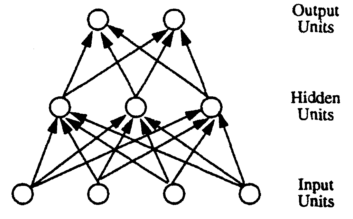
\includegraphics[]{net.png}
\caption{Multi-layer neural network with a single hidden layer.}
\end{figure}


\subsection{Perceptron}
%TODO ref on perceptrons
Activation functions can be linear or nonlinear.
A special kind of unit is the \textit{perceptron},
which outputs either a $-1$ or $1$,
depending on the value of a linear combination of the input:

\begin{equation}
\label{eq.perceptron}
o(\overrightarrow{x}) = \begin{cases}
1 & if \overrightarrow{w}\cdot\overrightarrow{x} > 0 \\
-1 & otherwise
\end{cases}
\end{equation}

\begin{figure}
\label{fig.ml.perceptron}
\center
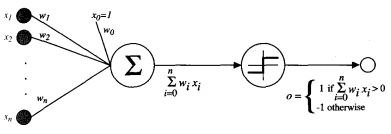
\includegraphics[]{perceptron.png}
\caption{Basic perceptron unit.}
%TODO accredit
\end{figure}

%TODO I have the perceptron img, need to clean and attribute properly
where $\overrightarrow{w}$ denotes the weights of the incoming connection
and $\overrightarrow{x}$ the corresponding incoming values.
This function effectively creates a hyperplane decision surface;
it separates the input space in two.

\subsection{Sigmoid}
A problem with perceptrons
is that they are not differentiable
in their whole domain.
As I'll explain further down, %TODO ref
differentiability is a useful and ofttimes required attribute.
As a way to circumvent this difficulty of non-differentiability,
the \textit{sigmoid} (denoted $\sigma(x)$) is often used:

\begin{equation}
\label{eq.ml.sigmoid}
\sigma(x) = \frac{1}{1 + e^{-x}}
\end{equation}

\begin{figure}[h]
\center
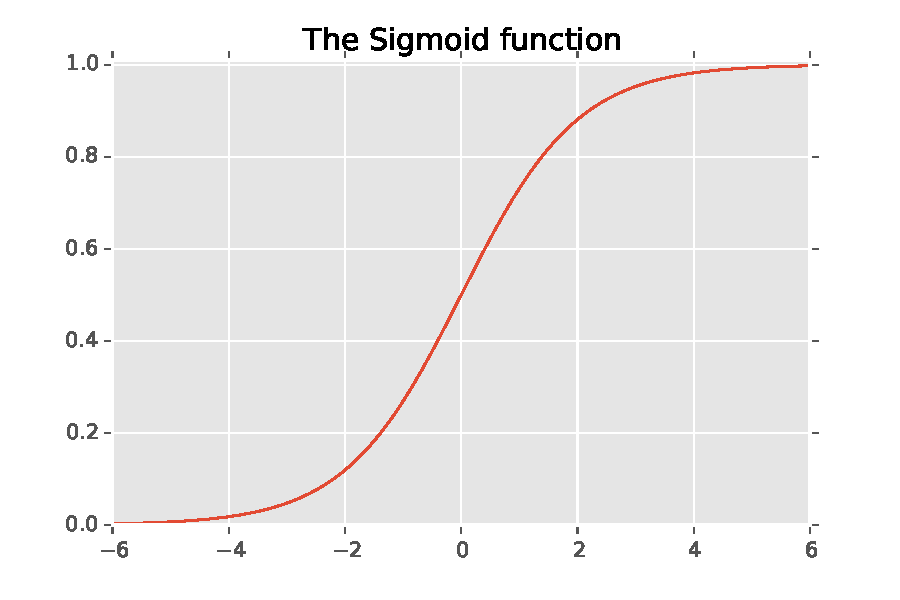
\includegraphics[width=.7\textwidth]{sigmoid.pdf}
\caption{The Sigmoid function}
\label{fig.ml.sigmoid}
\end{figure}

As can be seen on fig \ref{fig.ml.sigmoid},
it has the same tendency as the perceptron activation function
to separate the input space in two
but there is a transition area of uncertainty between the two extremes,
allowing the function to be differentiable in its whole domain.

In practice, the range is normalized between -1 and 1
just like the perceptron.

\subsection{Hyperbolic Tangent}
As a cousin to the sigmoid function, the hyperbolic tangent
deserves mentioning as well.
It bears the same shape as the sigmoid function
since it is really only a stretched
and shifted version.

\begin{equation}
\label{eq.ml.tanh}
\sigma(x) = \frac{1}{1 + e^{-2x}}+1
\end{equation}

\begin{figure}[h]
\center
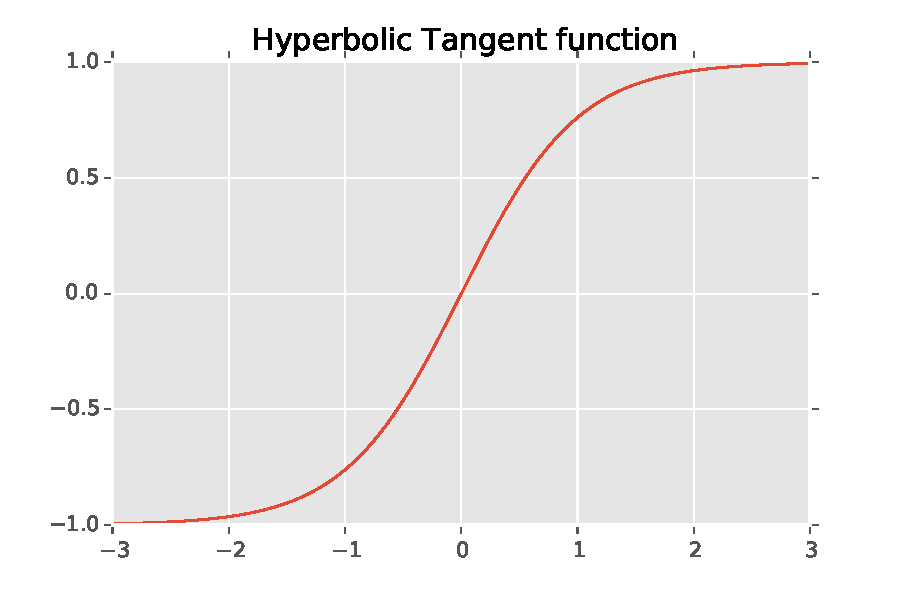
\includegraphics[width=.7\textwidth]{tanh.pdf}
\caption{The Sigmoid function}
\label{fig.ml.htan}
\end{figure}

\subsection{Rectified Linear Unit}
A fairly recent activation function is the
Rectified Linear Unit, or ReLU for short
\parencite{Nair2010}.

\begin{equation}
\label{eq.relu}
f(x) =
\begin{cases}
0 & \text{for } x < 0 \\
x & \text{for } x \geq 0
\end{cases}
\end{equation}

\begin{figure}[h]
\center
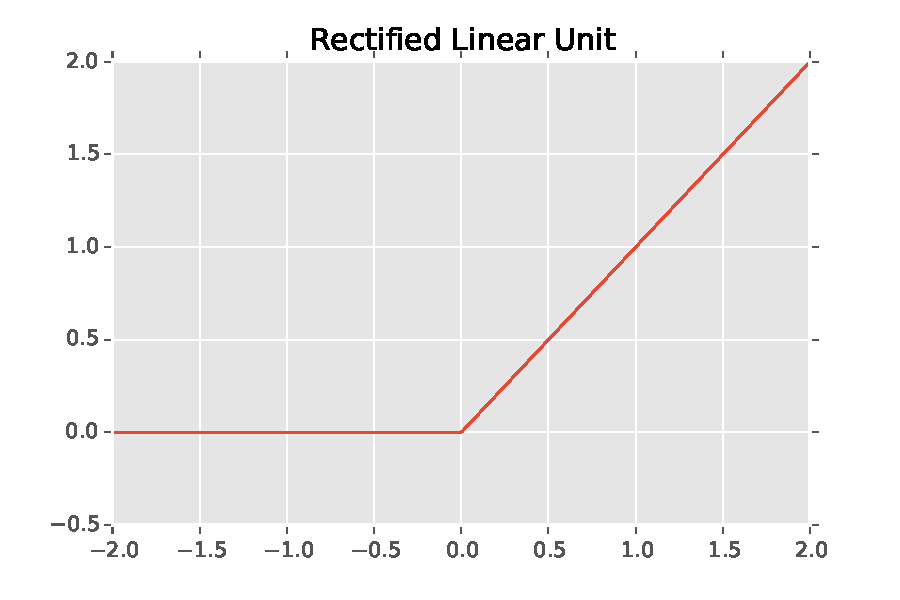
\includegraphics[width=.7\textwidth]{relu.pdf}
\caption{Rectified Linear Unit}
\label{fig.ml.relu}
\end{figure}

While it is very simple in its essence,
it has some important properties
that can be leveraged.
Among the advantages is that anything
below zero is mapped to zero.
This is great for sparse
network activations.
In a scenario with weights initialized
symmetrically (e.g. uniformly) around 0,
only half the neurons will activate.
This sparsity is great for discrimination
and effectively makes training
neural networks faster,
making it especially interesting for
deep learning
\parencite{Y.2015a}.

Linear rectifier functions also help mitigate
the \textit{vanishing gradient} problem %TODO consider ref'ing the vanishing gradient paper
since gradients above zero
are simply propagated.

\paragraph{}
The rectified unit family has gained quite some attention
ever since the first promising results.
Leaky rectified units comprise a subfamily
of functions that are designed to have a non-zero
gradient over their entire domain.
The basic version simply
has a fixed slope below zero
that is kept constant throughout training.

One such variant is the
\textit{Parametric rectified linear unit}
\parencite{He2015a},
a unit with a parametric slope below zero
that can be trained on data.

Another variant is the
\textit{Randomized rectified linear unit}
which has a randomized slope below zero.
The supposition is that the noise
will help prevent overfitting during training,
so the slopes are fixed outside of training.


\section{Gradient Descent and Backpropagation}
